\documentclass[a5paper,10pt,twoside,openany]{memoir}

% ============================================================
% A5 BOOKLET PRINTED ON FOLDED A4 SHEETS
% ============================================================
% The content is laid out as portrait A5 pages. In print mode,
% the booklet package places two A5 pages on each landscape A4
% side and rearranges the page order for folding and stapling.
%
% Recommended printer settings:
%   Paper size: A4
%   Orientation: Landscape
%   Duplex: On
%   Flip/bind: Short edge
%   Scaling: Actual size / 100 percent
% ============================================================

\newsavebox{\FrontImgBox}
\newlength{\FrontClip}

% ====== Fonts and language support ======
\usepackage[T1]{fontenc}
\usepackage[utf8]{inputenc}
\usepackage{microtype}
\usepackage{newtxtext}
\usepackage[scaled]{helvet}

% ====== Graphics, colour, columns, and boxes ======
\usepackage{float}
\usepackage{graphicx}
\usepackage{eso-pic}
\usepackage[dvipsnames]{xcolor}
\usepackage{tikz}
\usetikzlibrary{
  decorations.text,
  fadings,
  patterns,
  shapes.geometric
}

\usepackage{multicol}
\setlength{\columnsep}{5mm}
\setlength{\columnseprule}{0.2pt}

\usepackage{wrapfig}
\usepackage{caption}
\captionsetup{
  font=small,
  labelfont=bf
}
\captionsetup[figure]{
  labelformat=empty
}

\usepackage{lettrine}
\usepackage[many]{tcolorbox}
\usepackage{xparse}
\usepackage{contour}
\usepackage{pgfplots}
\pgfplotsset{
  width=9cm,
  compat=1.9
}

\usepackage{ifpdf}
\usepackage{todonotes}

% ====== True A5 page layout ======
% A5 is 148.5 mm wide by 210 mm high.
\settypeblocksize{178mm}{116mm}{*}
\setlrmarginsandblock{17mm}{15.5mm}{*}
\setulmarginsandblock{16mm}{16mm}{*}
\setheadfoot{12pt}{22pt}
\setheaderspaces{*}{6mm}{*}
\checkandfixthelayout

\raggedbottom

% ====== Booklet output switch ======
% Use \bookletprinttrue for a print-ready landscape A4 PDF.
% Use \bookletprintfalse for a normal sequential portrait A5 PDF.
\newif\ifbookletprint
\bookletprinttrue

% The booklet package must be loaded after the memoir page layout.
\ifbookletprint
  \usepackage[print,1to1]{booklet}
  \nofiles
\else
  \usepackage[noprint,1to1]{booklet}
\fi

% Source page: portrait A5.
% Target sheet: landscape A4.
\source{\magstep0}{148.5mm}{210mm}
\target{\magstep0}{297mm}{210mm}

% Each signature contains up to 16 A5 pages.
% Blank pages are added automatically when required.
\pagespersignature{16}

\ifpdf
  \setpdftargetpages

  % memoir resets the PDF page size at begin-document, so set
  % the physical output size again after memoir has finished.
  \ifbookletprint
    \AtBeginDocument{%
      \pdfpagewidth=297mm
      \pdfpageheight=210mm
    }
  \fi
\else
  \setdvipstargetpages
\fi

% Optional centre-fold guide.
% Change 0pt to 0.3pt to print a faint folding line.
\setlength{\pagesepwidth}{0pt}
\setlength{\pageseplength}{190mm}
\setlength{\pagesepoffset}{10mm}

\tcbset{
  colback=black!2,
  colframe=black!40,
  boxsep=4pt,
  left=6pt,
  right=6pt,
  top=6pt,
  bottom=6pt,
  sharp corners
}

% ====== Headings and bylines ======
\setsecheadstyle{\Large\bfseries\sffamily}
\setsubsecheadstyle{\normalsize\bfseries\sffamily}
\setsubsubsecheadstyle{\normalsize\itshape}

\newcommand{\kicker}[1]{%
  \textsf{\bfseries\small\color{Gray}#1}%
}

\newcommand{\headline}[1]{%
  \textsf{%
    \bfseries
    \fontsize{24}{26}\selectfont
    #1%
  }%
}

\newcommand{\deck}[1]{%
  \textsf{\normalsize\itshape #1}%
}

\newcommand{\byline}[1]{%
  \textsf{\small\color{Gray} Af #1}%
}

% ====== Image fading ======
\tikzfading[
  name=image fade,
  inner color=transparent!50,
  outer color=transparent!100
]

% ====== Text outline ======
\contourlength{0.9pt}
\contournumber{32}

\newcommand{\ow}[2][black]{%
  \contour{#1}{\textcolor{white}{#2}}%
}

\newcommand{\owthin}[2][black]{%
  \begingroup
  \contourlength{0.6pt}%
  \contour{#1}{\textcolor{white}{#2}}%
  \endgroup
}

% ====== Page banner and folio ======
\makepagestyle{newspaper}

\makeoddhead{newspaper}
  {\textsf{\scriptsize Den Rullende Sten}}
  {}
  {\textsf{\scriptsize Sponsoreret af Det Glemte Akademi}}

\makeevenhead{newspaper}
  {\textsf{\scriptsize Sponsoreret af Det Glemte Akademi}}
  {}
  {\textsf{\scriptsize Den Rullende Sten}}

\makeoddfoot{newspaper}
  {}
  {\textsf{\scriptsize\thepage}}
  {}

\makeevenfoot{newspaper}
  {}
  {\textsf{\scriptsize\thepage}}
  {}

\makeheadrule{newspaper}{\textwidth}{0.4pt}
\pagestyle{newspaper}

% ====== Pull quote environment ======
\newenvironment{pullquote}
  {%
    \begin{tcolorbox}[
      enhanced,
      breakable
    ]
    \itshape
    \large
  }
  {%
    \end{tcolorbox}
  }

% ====== Sidebar settings ======
\newcounter{sidebarlines}
\setcounter{sidebarlines}{14}
\setlength{\sidebarwidth}{0.42\columnwidth}

\newcommand{\godentry}[5]{%
  % #1 = placering
  % #2 = titel
  % #3 = billedfil
  % #4 = side l/r
  % #5 = tekst

  \begin{wrapfigure}{#4}{0.24\columnwidth}
    \vspace{-8pt}
    \centering
    \includegraphics[
      width=0.20\columnwidth
    ]{#3}
    \vspace{-12pt}
  \end{wrapfigure}

  \subsection*{#1. #2}

  #5

  \par\medskip
}

% ====== Utilities ======
\newcommand{\separator}{%
  \par
  \noindent
  {\color{black!40}\rule{\textwidth}{0.4pt}}
  \par
}

% ====== Front feature image ======
% Usage:
% \FrontFeatureImage
%   {image}
%   {kicker}
%   {headline}
%   {deck}
%   {credit}

\newcommand{\FrontFeatureImage}[5]{%
  % Typeset and measure the image.
  \sbox{\FrontImgBox}{%
    \includegraphics[
      width=0.94\textwidth
    ]{#1}%
  }%

  % Total scaled image height.
  \dimen0=\dimexpr
    \ht\FrontImgBox+
    \dp\FrontImgBox
  \relax

  % Maximum image height on an A5 page.
  \dimen2=.70\textheight

  % Select the visible height.
  \ifdim\dimen0>\dimen2
    \setlength{\FrontClip}{\dimen2}%
  \else
    \setlength{\FrontClip}{\dimen0}%
  \fi

  \begin{tikzpicture}
    % Image frame coordinates.
    \coordinate (TL) at (0,0);
    \coordinate (TR) at (\textwidth,0);
    \coordinate (BL) at (0,-\FrontClip);
    \coordinate (BR) at (\textwidth,-\FrontClip);

    % Image.
    \begin{scope}
      \clip (TL) rectangle (BR);

      \node[
        anchor=north west,
        inner sep=0pt,
        path fading=image fade,
        fit fading=false
      ] at (TL) {%
        \usebox{\FrontImgBox}%
      };
    \end{scope}

    % Dark overlay for text legibility.
    \begin{scope}
      \clip (TL) rectangle (BR);

      \fill[
        black,
        opacity=0.30,
        path fading=image fade
      ]
      (BL) rectangle (TR);
    \end{scope}

    % Headline stack.
    \node[
      anchor=south west,
      xshift=1em,
      yshift=1em,
      align=left,
      text width=.75\textwidth
    ] at (BL) {%
      \sffamily

      \if\relax\detokenize{#2}\relax
      \else
        {%
          \owthin[black!85]{%
            \textsf{\bfseries\small #2}%
          }%
        }\\[0.15em]
      \fi

      {%
        \ow{%
          \bfseries
          \resizebox{\textwidth}{!}{#3}%
        }%
      }\\[0.2em]

      {%
        \owthin{%
          \large
          \itshape
          #4%
        }%
      }%
    };

    % Image credit.
    \node[
      anchor=south east,
      xshift=-1em,
      yshift=1em
    ] at (BR) {%
      \sffamily
      \small
      \owthin[black!85]{#5}%
    };
  \end{tikzpicture}%
}

% ====== Information box ======
\newenvironment{infobox}[1]
  {%
    \begin{tcolorbox}[
      title=\textsf{\bfseries #1},
      colback=black!3,
      colframe=black!65,
      fonttitle=\small,
      fontupper=\small,
      boxsep=4pt,
      left=5pt,
      right=5pt,
      top=5pt,
      bottom=5pt,
      sharp corners
    ]
  }
  {%
    \end{tcolorbox}
  }

\newcommand{\paragraf}[1]{%
  \par
  \medskip
  \noindent
  \textbf{\S#1:}%
}

\begin{document}

% ============================================================
% FRONT PAGE
% ============================================================

\begin{center}
  
\includegraphics[
    width=0.98\textwidth
  ]{Logo.png}
\end{center}

\begin{center}
  {\Large\sffamily Udgave 135}
\end{center}

\FrontFeatureImage
  {SølvRavnen.png}
  {To nye guder dukker op}
  {Hvem er Sølvravnen og Den Grå Fyrste?}
  {"Har vi ophøjet to noble?"}
  {}

\vspace{.75\baselineskip}

\newpage

% ====== Lead story ======
\par\medskip
\headline{TO GUDINDER DØDE\\ TO NYE GUDER REJSTE SIG}
\par\medskip
\deck{Gudestenene krævede deres pris, mens mere end tyve ritualer ændrede gudernes sfærer.}
\par\medskip
\byline{Redaktionen}
\medskip

\begin{wrapfigure}[20]{r}{0.43\columnwidth}
\vspace{4pt}
\begin{infobox}{DET VED VI}
\begin{itemize}
\setlength{\itemsep}{0.25em}
\item Esselaia og Morwen er døde.
\item Morwen er blevet fuldstændigt udslettet.
\item Esselaias død menes at skabe Krigens Ærkedæmon.
\item Celina Coco er ophøjet som Sølvravnen.
\item Den Grå Fyrste er ophøjet som civilisationens og den sande adels gud.
\end{itemize}
\end{infobox}
\end{wrapfigure}

\lettrine[lines=2,lhang=0.1,loversize=0.05]{K}{alish}
har mistet to gudinder og fået to nye guder, men hvem er de og hvad førte til disse ukendte enheder blev ophøjet.

Begivenhederne begyndte ved Kaostræet for godt et år siden, hvor sortelvere ofrede fem væsner fra hver race og vandede træets rødder med deres blod. De håbede efter sigende at få del i træets magt.

I stedet blev gamle kræfter i A'kastin vækket.

På gudernes helliggrunde voksede de såkaldte Gudesten frem. Hver sten var forbundet til en gud, og kunne bruges til at påkalde den sagn-omspundende overguds magt til at dræbe en gud.

Oldstenene, som gudestenene også er kendt, var tidligere blevet brugt mod Daikia. Deres virkning var derfor kendt: Når stenene aktiveres, vil mindst én gud dø.

\subsection*{To gudinder rammes}

Nogle af stenene blev rettet mod Morwen, mens andre blev rettet mod Esselaia.

En tempelkriger i Morwens tjeneste valgte at rette sin sten mod Esselaia. Han håbede, at en ligelig fordeling ville gøre de to gudinder i stand til sammen at modstå stenenes kraft.

Det skete ikke, især da Morwen ikke var en sand gud, men en Ærkedæmon i forklædning.

Da gudinderne døde, forsvandt solen. Naturen skreg, tiden føltes forkert, og økonomien mistede den guddommelige orden, der hidtil havde understøttet den.

Morwen efterlod intet. Da hun allerede havde været en ærkedæmon før sin ophøjelse, kunne den normale forvandling ikke gentage sig. Hun blev i stedet fuldstændigt udslettet.

Esselaias skæbne er anderledes.

Inkvisitionen har ikke bekræftet noget, men tidligere undersøgelser i denne avis har beskrevet, hvordan en død gud kan blive til en ærkedæmon for det modsatte af sit vigtigste princip.

Esselaia var først og fremmest fredens gudinde.

Det, der følger efter hende, kendes derfor som \textbf{Krigens Ærkedæmon}.

\subsection*{Kampen om gudernes pladser}

Efter gudindernes død begyndte ophøjelsesritualerne.

På tre ritualpladser rundt omkring i A'kastin blev der gennemført mere end tyve mindre ritualer. Gamle artefakter kunne her binde guddommelige domæner til kandidaterne.

Mere end syv personer forsøgte at samle støtte.

Kong Dorian Vinterkrone støttede kandidater, der kunne gavne A'kastin og hans styre. Kejserinden ankom med egne ambitioner, mens både Elaith og efter sigende Hrothgar ligeledes forsøgte at gøre krav på guddommelig magt.

Da ritualerne sluttede, var det dog to helt andre skikkelser, der stod tilbage.

\subsection*{Sølvravnen rejser sig}

Den første var Celina Coco, bedre kendt som Sølvravnen.

Celina var leder af en gruppe dusørjægere og blev kendt for sin evne til at opspore Sølvfjend. Trods en næsten legendarisk gæld brugte hun sine penge på sit folk, særligt på musik, fornøjelser og hjælp til dem omkring sig.

Efter Esselaias død valgte dragerne at stille sig bag hende.

Celina blev ophøjet med \textbf{Omsorg} som sit overordnede princip og med domænerne \textbf{Musik}, \textbf{Drager} og \textbf{Natur}.

\begin{pullquote}
``Rigdom har kun værdi, når den skaber glæde for andre.''
- Celina Coco
\end{pullquote}

Sølvravnen står dermed som arvtager til flere af de områder, der blev efterladt tomme efter Esselaia.

\subsection*{Den Grå Fyrste rejser sig}

Den anden ophøjelse fik et langt mere uventet udfald.

Sortelvernes dronning forsøgte at tage den sidste guddommelige plads, men under det afsluttende ritual blev hun stukket ned af Den Grå Fyrste, som selv forsøgte at træde ind i hendes sted.

Med ham fulgte Lucius Krellenius.

Lucius havde gennem længere tid båret Den Grå Fyrstes kranie og lyttet til den gamle nekromantikers hvisken. Som fjerde søn af en gammel adelsslægt havde Lucius dog udviklet en helt anden forståelse af magt: Adel var for ham ansvar, værdighed og det eftermæle, man efterlader.

Da Den Grå Fyrste under ophøjelsen gav efter for sin gamle hunger efter magt og brutalitet, greb Lucius ind.

Han lod sig opsluge af Fyrsten og fyldte samtidig den guddommelige kraft med sine egne idealer.

Det ændrede den skikkelse, der rejste sig.

Den nye Grå Fyrste ønskede ikke længere at herske over de døde. I stedet vendte hans blik sig mod de dødelige: deres historier, deres samfund og det, de formår at bygge og efterlade.

Den Grå Fyrste er derfor blevet gud for \textbf{Civilisation}, \textbf{Strategi}, \textbf{Adel} og \textbf{Døden}.

\begin{pullquote}
``Skab dig et eftermæle, noget der overlever dig. Den enkelte dør, men værker består.''
- Den Grå Fyrste
\end{pullquote}

\subsection*{En ny guddommelig orden}

Kalish står derfor tilbage med to nye guder, der næppe kunne være mere forskellige.

Sølvravnen lærer sine tilbedere at passe på deres folk, dele deres rigdom og lade musik og natur skabe glæde.

Den Grå Fyrste lærer dem at bygge noget, der varer længere end deres eget liv, og at forstå magt som ansvar.

Men sejren har haft en pris.

Morwen findes ikke længere.

Esselaia er død.

Og hvis undersøgelserne af hendes skæbne er korrekte, er fredens tidligere gudinde nu ved at blive til noget, som Kalish endnu ikke har mødt:

Krigens Ærkedæmon.

\separator

\par\medskip

\textit{Redaktionen modtager oplysninger om Sølvravnens og Den Grå Fyrstes nye præster, templer og varsler. Som altid accepteres anonyme henvendelser.}


% ====== Bekendtgørelse fra Sølvhammerens Orden ======

\begin{center}
\begin{tcolorbox}[
  enhanced,
  width=0.94\textwidth,
  colback=black!2,
  colframe=black!85,
  boxrule=1.4pt,
  breakable,
  borderline={0.7pt}{3pt}{Goldenrod!70!black},
  sharp corners,
  boxsep=2mm,
  left=7mm,
  right=7mm,
  top=5mm,
  bottom=5mm,
  overlay={
    % Dekorative hjørner
    \draw[Goldenrod!75!black,line width=1.2pt]
      ([xshift=2mm,yshift=-2mm]frame.north west)
      -- ++(14mm,0) -- ++(0,-7mm);

    \draw[Goldenrod!75!black,line width=1.2pt]
      ([xshift=-2mm,yshift=-2mm]frame.north east)
      -- ++(-14mm,0) -- ++(0,-7mm);

    \draw[Goldenrod!75!black,line width=1.2pt]
      ([xshift=2mm,yshift=2mm]frame.south west)
      -- ++(14mm,0) -- ++(0,7mm);

    \draw[Goldenrod!75!black,line width=1.2pt]
      ([xshift=-2mm,yshift=2mm]frame.south east)
      -- ++(-14mm,0) -- ++(0,7mm);
  }
]

\begin{center}

{\sffamily\bfseries\small\color{black!65}
OFFICIEL BEKENDTGØRELSE}

\vspace{0.25em}

{\sffamily\bfseries\fontsize{27}{29}\selectfont
SØLVHAMMERENS ORDEN}

\vspace{0.2em}

{\sffamily\bfseries\large
TIL BORGERNE I A'KASTIN}

\vspace{0.35em}

{\color{Goldenrod!75!black}
\rule{0.78\linewidth}{1.2pt}}

\end{center}

\vspace{0.6em}

\lettrine[lines=1,lhang=0.1,loversize=0.05]{B}{orgere} i A'kastin!

Vi, \textbf{Sølvhammerens Orden}, har igennem det sidste år
øget vores tilstedeværelse i A'kastin som et led i forsvaret af
Kelllwan Kirkens tjenere, troende og riget.

Vort fokus har været at standse de dæmoniske trusler, der har
bragt alle vores liv i fare. Under ledelse af
\textbf{Ordensmester Seiger} har vi bekæmpet enhver fjende,
der har truet dem, vi har svoret at beskytte.

Vores ridderorden er grundlagt for at beskytte
\textbf{Kelllwan-troende}, \textbf{Kelllwans præsteskab},
rigerne under Kelllwans åsyn og alle lovlydige borgere.

Den største sejr, vi har været med til at frembringe, har været
\textbf{genopbygningen af Sydporten}.

Gennem vores forbindelser til Kelllwan Kirken og et omfattende
samarbejde med utallige modige borgere i A'kastin er det
lykkedes at samle de nødvendige ressourcer og igen rejse
Sydporten til rigets forsvar.

\vspace{0.5em}

\begin{tcolorbox}[
  colback=Goldenrod!7,
  colframe=Goldenrod!65!black,
  boxrule=0.8pt,
  sharp corners,
  title={\sffamily\bfseries EN SÆRLIG TAK},
  colbacktitle=black!85,
  coltitle=white,
  fontupper=\small,
  left=4mm,
  right=4mm,
  top=3mm,
  bottom=3mm
]

Sølvhammerens Orden ønsker særligt at takke de personer og
organisationer, der hjalp med at indsamle ressourcerne til
genopbygningen:

\begin{itemize}
  \setlength{\itemsep}{0.35em}

  \item \textbf{Præstinde Halborg Ragnhild Borgesdatter af Halvvog},
        præstinde for Kelllwan.

  \item \textbf{Kong Dorian af A'kastin}.

  \item \textbf{Esselaia Kirken}

  \item De utallige \textbf{frivillige borgere og indbyggere},
        som gav deres tid, styrke og ressourcer.

  \item \textbf{Handelskompagniet}.
\end{itemize}

\end{tcolorbox}

\vspace{0.6em}

Sølvhammerens Orden vil fortsætte arbejdet med at bekæmpe
dæmonerne og holde riget frit.

\vspace{0.8em}

\begin{center}

{\color{Goldenrod!75!black}
\rule{0.55\linewidth}{1pt}}

\vspace{0.5em}

{\sffamily\bfseries\Large
HIL KELLLWAN}

\vspace{0.25em}

{\sffamily\small\itshape
Sølvhammerens Orden}

\end{center}

\end{tcolorbox}
\end{center}


% ====== Rohar advertisement ======
\begin{center}
  \begin{tcolorbox}[
    enhanced,
    breakable,
    width=0.94\textwidth,
    colback=ForestGreen!4,
    colframe=black,
    boxrule=1.4pt,
    borderline={
      0.7pt
    }{
      3pt
    }{
      ForestGreen!70!black
    },
    sharp corners,
    boxsep=2mm,
    left=5mm,
    right=5mm,
    top=4mm,
    bottom=3mm,
    overlay={
      % Top-left ornament.
      \draw[
        ForestGreen!70!black,
        line width=1.2pt
      ]
      ([xshift=2mm,yshift=-2mm]frame.north west)
      -- ++(11mm,0)
      -- ++(0,-7mm);

      % Top-right ornament.
      \draw[
        ForestGreen!70!black,
        line width=1.2pt
      ]
      ([xshift=-2mm,yshift=-2mm]frame.north east)
      -- ++(-11mm,0)
      -- ++(0,-7mm);

      % Bottom-left ornament.
      \draw[
        ForestGreen!70!black,
        line width=1.2pt
      ]
      ([xshift=2mm,yshift=2mm]frame.south west)
      -- ++(11mm,0)
      -- ++(0,7mm);

      % Bottom-right ornament.
      \draw[
        ForestGreen!70!black,
        line width=1.2pt
      ]
      ([xshift=-2mm,yshift=2mm]frame.south east)
      -- ++(-11mm,0)
      -- ++(0,7mm);
    }
  ]

    \begin{center}
      {%
        \sffamily
        \bfseries
        \small
        TRÆT AF SVAGE GUDER OG TOMME LØFTER?%
      }

      \vspace{0.15em}

      {%
        \sffamily
        \bfseries
        \fontsize{22}{24}\selectfont
        \textcolor{ForestGreen!55!black}{%
          REJS DIG FOR ROHAR!%
        }%
      }

      \vspace{0.1em}

      {%
        \sffamily
        \bfseries
        \large
        KONGEN - DEN DER KOM TILBAGE%
      }
    \end{center}

    \vspace{0.5em}

    \noindent
    \colorbox{black}{%
      \parbox{\dimexpr\linewidth-2\fboxsep\relax}{%
        \centering
        \color{white}
        \itshape
        \large

        ``Før var jeg træt og deprimeret, men så prøvede jeg
        at tilbede Rohar. Nu har jeg styrke, et formål og en
        gud, der råber gode råd gennem min økse!''

        \normalfont
        \small

        - Gruk Jernpande, tidligere Orlek Præst
      }%
    }

    \vspace{0.7em}

    \begin{center}
      \colorbox{ForestGreen!70!black}{%
        \parbox{0.88\linewidth}{%
          \centering
          \color{white}
          \sffamily
          \bfseries
          \large

          SPØRG EFTER ROHAR PRÆSTEN ELLER TEMPELKRIGEREN
          HVIS DU GERNE VIL VIDE MERE!

          \smallskip

          \normalsize

          Medbring jern, og alle dine fjend for at vise
          at du er værdig.
        }%
      }
    \end{center}

    \vspace{0.4em}

    \begin{center}
      {%
        \sffamily
        \bfseries
        ROHAR DØDE. DET STOPPEDE HAM IKKE.\\
        HVAD ER DIN UNDSKYLDNING?%
      }
    \end{center}

  \end{tcolorbox}
\end{center}

% ============================================================
% ADVERTISEMENTS
% ============================================================

% ====== Handelskompagniets Kongetand-reklame ======
\begin{figure}
  \centering
  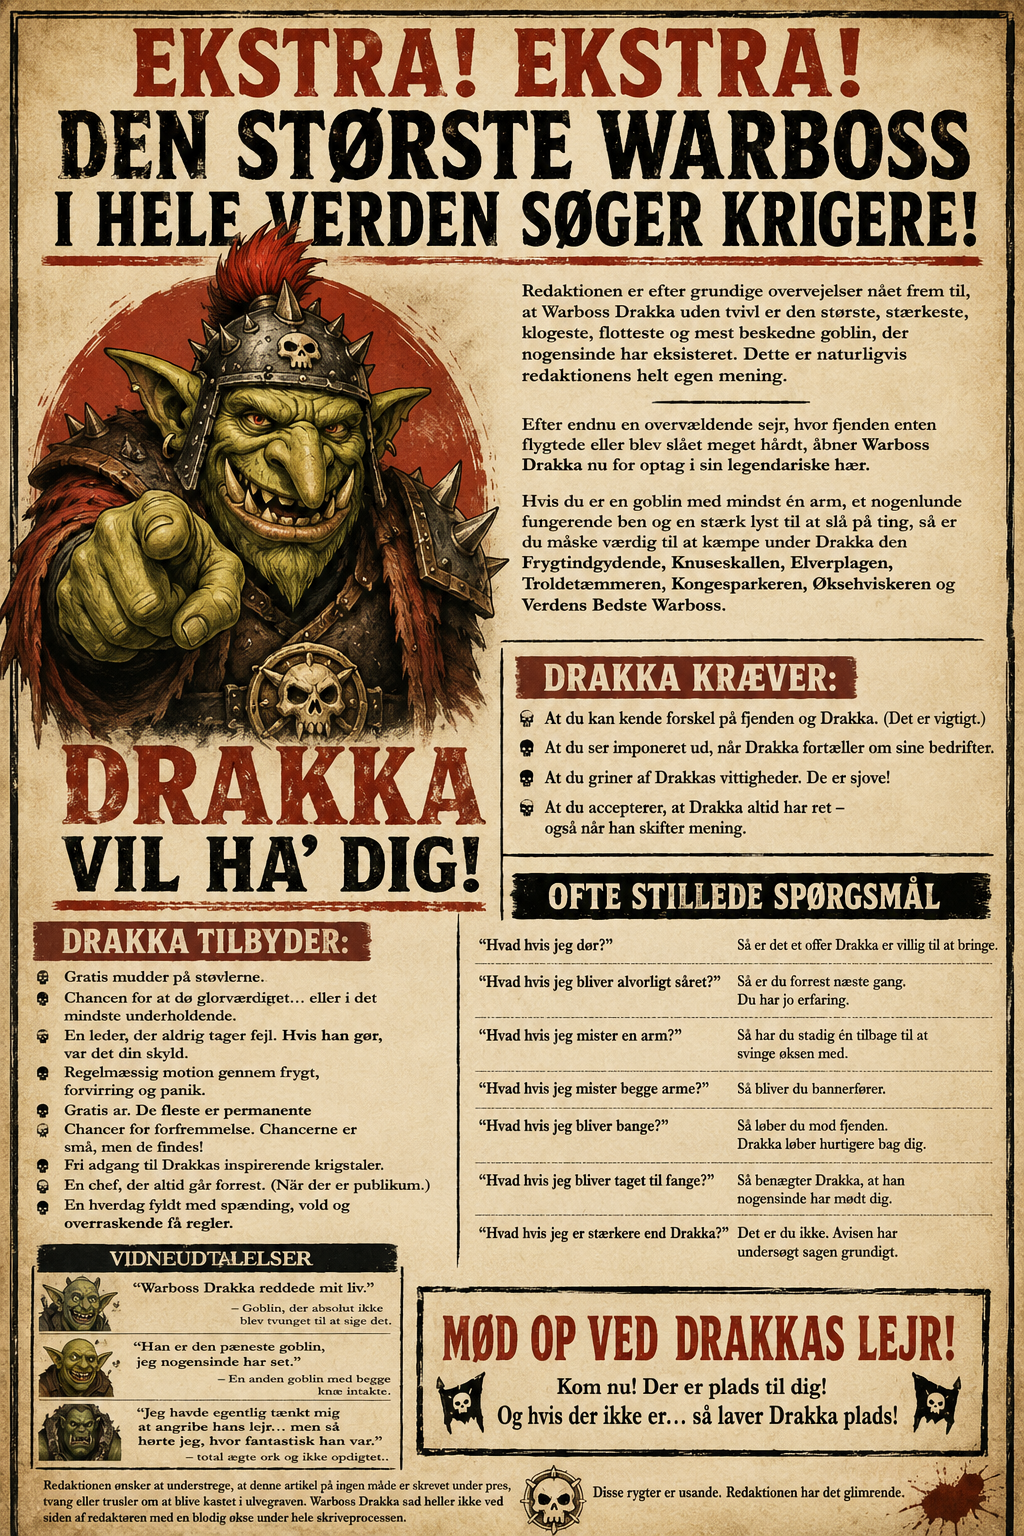
\includegraphics[width=0.98\textwidth]{Drakka.png}
\end{figure}

\begin{figure}
  \centering
  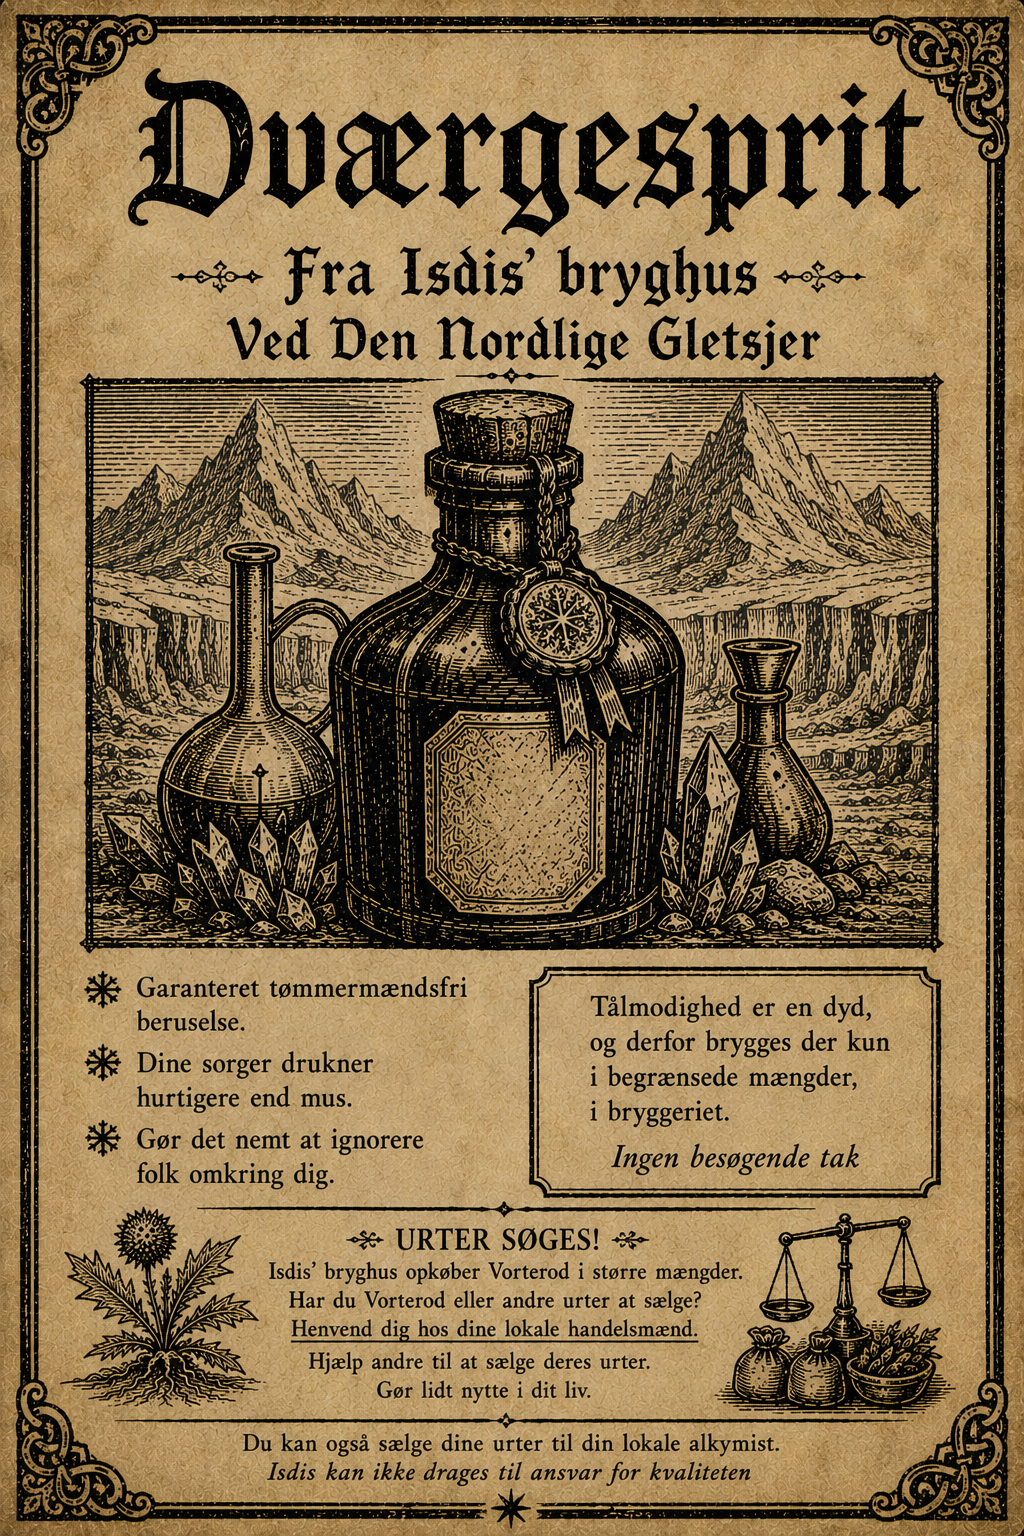
\includegraphics[width=0.98\textwidth]{Dværgesprit.png}
\end{figure}


\vspace*{\fill}

\clearpage

\end{document}